% Template FILKOM UB: lihat TEMPLATE-UB.md untuk asal dan adaptasi.
% Calibri asli: XeLaTeX + Biber; format lainnya di gaya/ubtesis.sty.
\documentclass[12pt,a4paper,oneside]{report}
\usepackage{gaya/ubtesis}
\addbibresource{bibliography.bib}
% Basis .bib dibagi dengan Beamer lama; n.d. adalah penanda tahun tak diketahui,
% bukan tahun rekaan. Untuk Biber, hilangkan field itu agar gaya mencetak t.t.
\DeclareSourcemap{\maps[datatype=bibtex]{\map{
  \step[fieldsource=year,match=\regexp{\An\.d\.\z},final]
  \step[fieldset=year,null]}}}
\hypersetup{pdftitle={Pemodelan Smart Traffic Light dengan MBSE dan SysML 1.6},
  pdfauthor={Edy Rahman; Ramadhani Al-Qadri}}
\graphicspath{{gambar/}{../assets/diagrams/}}
% Metadata sampul laporan proyek; program studi mengikuti konteks MILKOM.
\newcommand\judul{Pemodelan Smart Traffic Light Berbasis Kepadatan Kendaraan dengan Pendekatan Model-Based Systems Engineering}
\newcommand\jenisnaskah{LAPORAN PROYEK}
\newcommand\penulis{Edy Rahman (256150100011007)\\Ramadhani Al-Qadri (256150100011010)}
\newcommand\programstudi{PROGRAM STUDI MAGISTER ILMU KOMPUTER}
\newcommand\departemen{DEPARTEMEN TEKNIK INFORMATIKA}
\newcommand\fakultas{FAKULTAS ILMU KOMPUTER}
\newcommand\universitas{UNIVERSITAS BRAWIJAYA}
\newcommand\kota{MALANG}
\newcommand\tahun{2026}

\begin{document}
\margininduk
\pagenumbering{roman}
% Adaptasi blok penyusun untuk dua anggota; nama dan NIM berpasangan di metadata.
% Sampul [spek D]. Tanpa nomor halaman, tetapi terhitung sebagai halaman i.
% Jarak vertikal disetel terhadap Template Tesis V2.pdf hal-1; lihat _verifikasi/v2/.
% Judul panjang akan menambah baris dan menggeser blok atas ke bawah,
% sama seperti di Word; blok institusi tetap tertambat di bawah.
\begin{titlepage}
\thispagestyle{empty}
\setlength{\parskip}{0pt}
\centering
\vspace*{-0.57cm}  % V2: garis dasar judul 4,04 cm dari tepi atas
{\bfseries\ukuran{16}\judul\par}   % V2: 16 pt tebal, huruf judul (Title Case), bukan kapital
\vspace{0.89cm}
{\bfseries\ukuran{14}\jenisnaskah\par}              % AcademicLevel 14 pt tebal
\vspace{2.55cm}
{\ukuran{14}Disusun oleh:\par
 \penulis\par}
\vspace{2.72cm}  % V2: logo 5 cm, tepi atas 14,71 cm

\includegraphics[width=5cm]{logo-ub}\par
\vfill
{\ukuran{14}\programstudi\par
 \departemen\par
 \fakultas\par
 \universitas\par
 \kota\par
 \tahun\par}
\vspace{0.16cm}  % V2: garis dasar tahun 26,54 cm dari tepi atas
\end{titlepage}
\setcounter{page}{2}

\babtanpanomor{Ringkasan}
Proyek ini merancang model konseptual pengendali sinyal untuk satu simpang empat pendekat. Model menerima jumlah kendaraan, mengelompokkan kondisi traffic, memilih pendekat yang belum dilayani pada putaran berjalan, serta mengunci durasi hijau menurut kategori. Evidence dari dua artikel traffic, satu kajian MBSE dan catatan kuliah dipisahkan dari asumsi desain kelompok. Tujuh view Systems Modeling Language (SysML) direpresentasikan melalui Mermaid dan PlantUML sebagai renderer tekstual. Sebanyak 24 requirement dihubungkan dengan perilaku, komponen dan 21 skenario verifikasi. Analisis referensi terhadap 576 pasangan urutan dua putaran menghasilkan batas tunggu maksimum 208 detik pada asumsi nominal, di bawah batas desain 210 detik. Angka tersebut merupakan hasil analisis kontrak penjadwalan, bukan pengukuran kinerja traffic, delay kendaraan atau bukti keselamatan perangkat fisik. Perilaku fault dan recovery yang belum dieksekusi tetap ditandai belum diuji.

\daftarisi
\daftartabel
\daftargambar
\marginisi
\clearpage
\pagenumbering{arabic}
\chapter{Pendahuluan}
\section{Latar belakang}
Tugas yang dicatat pada materi kuliah meminta sistem yang mendeteksi kondisi kendaraan dan memberikan hijau lebih lama kepada ruas dengan kondisi lebih padat \parencite[bagian 21]{lecture02}. Penyesuaian fase dan durasi merupakan dua keputusan yang berbeda. \textcite{mondal2022} menggunakannya dalam rancangan adaptive control berbasis density dan waiting time, sedangkan \textcite{mathiane2023} menggabungkan penghitungan kendaraan, klasifikasi dan pengaturan sinyal. Rancangan proyek mengambil rationale input dan kontrol adaptif tanpa mewajibkan seluruh teknologi kedua artikel.

Pemodelan perlu menjelaskan batas sistem, tanggung jawab komponen, transisi sinyal, dan cara memeriksa kebutuhan. Catatan kuliah menekankan consistency dan traceability antar-view \parencite[bagian 9--10]{lecture01}. Pada proyek ini, hubungan evidence/asumsi, requirement, behavior, structure dan verification menjadi dasar audit desain; keberadaan diagram saja belum membuktikan peningkatan throughput.

\section{Rumusan masalah dan tujuan}
Masalah desain adalah bagaimana merepresentasikan pengendali empat pendekat yang adaptif, tidak memberi green berkonflik, mempunyai batas pelayanan dan perilaku data-failure yang jelas. Tujuannya menghasilkan model subset SysML 1.6 yang konsisten, katalog requirement yang dapat diperiksa, serta skenario verifikasi dengan status pelaksanaan yang jujur. Laporan dan presentasi merupakan artefak akademik, bukan perangkat pengendali lapangan.

\section{Metode pengerjaan}
Urutan kerja adalah audit sumber, kajian terarah tiga jurnal yang dipilih pengguna, pencatatan evidence/asumsi, formulasi masalah, requirements, behavioral/structural views, traceability dan analisis verifikasi. Kajian ini bukan pencarian literatur exhaustif atau systematic review baru. Identitas sumber dan konteks klaim diperiksa sebelum dipakai. Bantuan kecerdasan buatan (artificial intelligence, AI) digunakan untuk ekstraksi, penyusunan source, dan pemeriksaan; tanggung jawab peninjauan akademik tetap pada kelompok.


\section{Konvensi identitas}
ID berarti identifier elemen yang stabil. Prefiks EVID menandai evidence, ASM asumsi desain, REQ requirement, UC use case, ACT action, BLK block, VER verification/test case, STM state machine, dan INT interaction. Pada evidence, TRF berarti traffic, LEC catatan lecture, dan MBSE kajian metodologis. LOW, MEDIUM dan HIGH merupakan label enumeration kategori, bukan singkatan bebas. Nomor dan identitas tetap sama lintas source serta diagram.

\chapter{Landasan Teori dan Studi Literatur}
\section{MBSE dan SysML}
Materi kuliah menggambarkan MBSE sebagai pendekatan rekayasa yang memusatkan requirement, desain, analisis dan verification pada model yang saling terhubung \parencite[bagian 3 dan 10]{lecture01}. SysML digunakan untuk menyatakan konsep model, sedangkan Mermaid dan PlantUML hanya merender representasi tekstual. Versi 1.6 dipilih sebagai asumsi proyek ASM-010; catatan kuliah tidak menyatakan nomor versi. Referensi normatif tambahan adalah \textcite{omg2019}.

Subset mencakup Requirement, UseCase, Activity/Action, Interaction/Message, StateMachine, Block, PartProperty, ProxyPort, InterfaceBlock, Connector/ItemFlow serta dependency satisfy, verify dan allocate. Block Definition Diagram (BDD) memuat definisi tipe; Internal Block Diagram (IBD) memuat penggunaan part di dalam context block. Relasi satisfy berarah dari elemen pemenuh ke requirement, verify dari test case ke requirement, dan allocate dari elemen yang dialokasikan ke target alokasi \parencite[bagian 15.3.1.2, 16.3.2.7, 16.3.2.9]{omg2019}. Model tidak diklaim telah diperiksa melalui engine SysML atau seluruh constraint Object Constraint Language (OCL).

\section{Artikel traffic pertama}
\textcite{mondal2022} merancang prioritas berbasis kombinasi density dan waiting time, serta green time proporsional terhadap density (PDF 3--5; EVID-TRF-001). Input contoh memakai jumlah mobil dan waiting time; output berupa urutan fase dan timer. Sensor, road-side unit (RSU), processing unit dan traffic light controller dipisahkan (EVID-TRF-002). Simulasi Python membandingkan kondisi balanced/unbalanced dengan fixed-time. Peningkatan average percentage traffic flow yang dilaporkan 31.05\% adalah hasil studi tersebut, bukan hasil proyek ini (PDF 8--9; EVID-TRF-005).

Ada keterbatasan yang harus dipertahankan dalam interpretasi. Algorithm 1 baris 6 memakai ascending order, sementara contoh Table 1 memilih prioritas terbesar (PDF 6; EVID-TRF-004). Rumus normalisasi dengan penyebut max-minus-min juga membutuhkan aturan tambahan saat semua nilai sama; ini analisis atas rumus, bukan laporan kegagalan simulator penulis. Karena itu kontrak scheduler proyek tidak menyalin pseudocode artikel secara langsung.

\section{Artikel traffic kedua}
\textcite{mathiane2023} memakai hitungan kelompok kendaraan, two-dimensional convolutional neural network (2D-CNN), simulasi Pygame dan pembanding Simulation of Urban Mobility (SUMO). Density pada bagian 3.1 dihitung menggunakan jumlah kendaraan serta konfigurasi lajur; definisinya bukan normalisasi kapasitas pendekat proyek (EVID-TRF-006). Input klasifikasi dan input kontrol dibedakan. Baseline dapat menerima hitungan yang sudah tersedia tanpa membuat training pipeline kamera.

Angka klasifikasi 96\% merujuk pengenalan jenis kendaraan, bukan keselamatan controller. Abstrak memakai istilah 90\% throughput, sementara kesimpulan memakai 90\% faster (EVID-TRF-008). Kajian tidak mengharmonisasi keduanya menjadi target numerik. Hardware dan deteksi malfunction masih disebut sebagai pengembangan berikutnya; artikel tidak membuktikan fail-safe proyek siap digunakan (bagian 5; EVID-TRF-007).

\section{Artikel MBSE dan batas evidence}
\textcite{campo2023} melakukan analisis konten terhadap 2914 klaim dari 60 sumber. Temuannya membahas persepsi manfaat, drawback, evidence dan metrik, bukan eksperimen kausal pada satu pengendali. Penulis melaporkan 47\% klaim berbasis author opinions dan 86\% tidak disubstansiasi metrik (Abstract, bagian 3.2 dan 3.3.6; EVID-MBSE-001/002). Ini mendukung kehati-hatian terhadap klaim manfaat MBSE, bukan angka keberhasilan proyek.

Pemilihan corpus studi Campo tidak exhaustif dan bagian 2.1 menyatakan tidak menilai mutu metodologi setiap sumber. PDF lokal memiliki peringatan xref meskipun 26 halaman terbaca; locator bagian digunakan tanpa mengklaim integritas page-anchor lulus. Kedua PDF traffic lulus structural preflight. Metadata Springer cocok dengan PDF; akses MDPI mendapat 429 dan permintaan Wiley lanjutan mendapat 403. Batas ini dicatat tanpa mengganti sumber pengguna.

\section{Sintesis untuk rancangan}
Kedua studi traffic memberi dasar konsep adaptasi green terhadap kondisi kendaraan. Perbedaan formulasi, teknologi dan lingkup emergency tidak dijadikan kewajiban untuk menggabungkan semua fitur. Materi kuliah memberi dasar hubungan antar-view; kajian MBSE memberi batas terhadap klaim manfaat yang tidak diukur. Aturan tie-break, hard waiting bound, sampling, kategori dan failure handling spesifik tetap merupakan asumsi desain kelompok. Register evidence penuh berada pada source penelitian repository; Tabel~\ref{tab:evidence} merangkum lokasi dan penggunaannya.
\begin{longtable}{|>{\raggedright\arraybackslash}p{.17\linewidth}|>{\raggedright\arraybackslash}p{.27\linewidth}|>{\raggedright\arraybackslash}p{.43\linewidth}|}
\caption{Ringkasan evidence dan batas penggunaannya}\label{tab:evidence}\\
\hline
\textbf{ID} & \textbf{Lokasi sumber} & \textbf{Penggunaan / batas} \\ \hline
\endfirsthead
\lanjutan{3}
\hline
\textbf{ID} & \textbf{Lokasi sumber} & \textbf{Penggunaan / batas} \\ \hline
\endhead
TRF-001 & Mondal PDF 3--5 & Input, prioritas, green adaptif; bukan tie-break proyek \\ \hline
TRF-002 & Mondal PDF 3--4 & Tanggung jawab komponen dan empat fase \\ \hline
TRF-003 & Mondal PDF 5--6 & Inventaris angka sumber; tidak otomatis diadopsi \\ \hline
TRF-004 & Mondal PDF 6 & Disposition perbedaan pseudocode/contoh \\ \hline
TRF-005 & Mondal PDF 8--9 & Skenario balanced/unbalanced; hasil hanya milik studi \\ \hline
TRF-006 & Mathiane 3.1 & Hitungan sebagai input; definisi density khusus studi \\ \hline
TRF-007 & Mathiane 3.2 dan 5 & Lingkup CNN/emergency dan hardware future work \\ \hline
TRF-008 & Mathiane abstrak dan 5 & Istilah hasil kuantitatif berbeda; tidak jadi target \\ \hline
MBSE-001 & Campo 2.1--2.2 & Metode/corpus dan batas evidence \\ \hline
MBSE-002 & Campo 3.2, 3.3.6, 4 & Bedakan persepsi, bukti dan metrik \\ \hline
LEC-001 & Catatan 01:9--10; 02:16--19 & Consistency dan traceability \\ \hline
LEC-002 & Catatan 02:5 & Requirement, satisfy, verify \\ \hline
LEC-003 & Catatan 02:7--9 & Tiga sudut behavior \\ \hline
LEC-004 & Catatan 02:10--13 & BDD type, IBD part/port/connector \\ \hline
LEC-005 & Catatan 02:21 & Tujuan tugas; provenance slide belum dicocokkan \\ \hline
\end{longtable}
\sumber{Olahan kajian berdasarkan \textcite{mondal2022,mathiane2023,campo2023} dan catatan kuliah}

ID pada tabel memakai prefiks lengkap EVID-. Catatan kuliah disediakan sebagai Markdown yang diperluas dari slide; penulis, tanggal, institusi dan batas perluasan tidak dicantumkan. Kutipan mengacu ke catatan yang tersedia, bukan mengarang identitas dosen atau nomor slide asli \parencite{lecture01,lecture02}.

\chapter{Analisis Permasalahan dan Asumsi Desain}
\section{Scope, stakeholder dan input}
System of Interest adalah SmartTrafficLightSystem dengan pendekat North, South, East, West, hanya gerak lurus. Tidak ada pedestrian, dedicated turn, emergency, dashboard, machine learning (ML) atau koordinasi antarsimpang. Baseline mengeksekusi satu green pada satu waktu; setiap pasangan pendekat berbeda dianggap berkonflik secara konservatif. TrafficDataSource adalah aktor eksternal penyedia hitungan, RoadUsers penerima sinyal, sedangkan kelompok/dosen meninjau artefak dan pengelola lalu lintas berkepentingan terhadap batas desain.

VehicleDetection adalah adapter input, bukan sensor kamera yang telah diimplementasikan. CountsFrame berisi empat record dengan approach unik, vehicleCount integer 0 sampai 2147483647, observedAt pada clock monotonic bersama, dan flag valid. Hitungan adalah snapshot antrean pada akhir jendela observasi, bukan kendaraan lewat per detik atau kendaraan/km. Kapasitas dan area fisik lokasi tidak tersedia; belum ada kalibrasi.

\begin{table}[htbp]\centering
\caption{Parameter baseline: seluruhnya asumsi desain ASM-002--008}
\begin{tabular}{|p{.43\linewidth}|p{.44\linewidth}|}
\hline
\textbf{Parameter} & \textbf{Nilai / aturan} \\ \hline
Kategori LOW / MEDIUM / HIGH & 0--5 / 6--15 / $\geq 16$ kendaraan \\ \hline
Green LOW / MEDIUM / HIGH & 10 / 20 / 30 s \\ \hline
Minimum / maximum green & 10 / 30 s \\ \hline
Yellow / all-red & 3 / 1 s \\ \hline
Observasi / decision tick & 1 / 1 s \\ \hline
Stale threshold & umur $>3$ s \\ \hline
Maximum service waiting & 210 s, operasi round baseline \\ \hline
Fallback / recovery & green 10 ring / 3 frame baru baik + round baru \\ \hline
\end{tabular}
\sumber{Asumsi desain proyek ASM-002--008 (2026)}\end{table}

Angka artikel seperti cycle 120 s atau amber 2.5 s pada Mondal tidak menetapkan parameter lokasi proyek. Nilai tabel dipilih sebagai grid konseptual yang mudah dianalisis; tidak diklaim aman untuk geometri persimpangan tertentu. Dua hitungan dalam kategori sama boleh mendapat grant sama. Setiap perubahan parameter memerlukan perhitungan ulang bound dan revisi artefak.

\section{Prioritas dan batas tunggu}
Setiap pendekat mendapat satu pelayanan dalam setiap round, termasuk count nol. Eligible hanya memuat pendekat yang belum dilayani pada round berjalan. Pada akhir all-red, urutan nominal adalah kategori menurun, waktu tunggu menurun, lalu ring N--S--E--W dengan pointer awal N. Pointer maju ke penerus pendekat yang baru menerima green. Grant aktif tidak diubah oleh sampel baru.

Waktu tunggu diukur sejak green pendekat terakhir berakhir dan nol selama green; untuk pendekat belum pernah dilayani diinisialisasi dari startup. Ini waktu menunggu kesempatan pelayanan, bukan delay tiap kendaraan. Rencana sisa round diperiksa terhadap deadline 210 s; bila urutan nominal melampauinya, earliest-deadline-first (EDF) mengambil alih. Rencana yang tetap tidak layak meminta SafetyHold.

Pada dua round bersebelahan, suatu pendekat dapat berpindah dari pertama menjadi terakhir. Paling banyak enam green lain dan tujuh clearance berada di antaranya:
\begin{equation}\label{eq:bound}
W_{\max}\leq 6G_{\max}+7(Y+A)=6(30)+7(3+1)=208\ \mathrm{s}<210\ \mathrm{s}.
\end{equation}
Startup terburuk bagi pendekat terakhir adalah $1+3(30+4)=103$ s. Margin 2 s merupakan margin diskrit model, bukan allowance latensi perangkat nyata.

\section{Failure handling dan batas jaminan}
Cache fresh boleh digunakan saat satu event sampel hilang. Frame invalid, valid=false, cache tidak lengkap atau stale melatch dataFault; count salah tidak diganti nol. Fault data tidak memotong grant aktif. Sesudah green dan clearance selesai, Fallback melayani eligible dalam ring dengan green 10. Round dan wait timers tidak direset saat pergantian mode. Adapter mengecek cache tiap tick walau input berhenti. Latch sensor clear setelah tiga frame baru baik, tetapi mode Fallback ditahan sampai round baru. Pemulihan membutuhkan tiga frame lengkap valid dengan timestamp baru berturut-turut pada tick berbeda, lalu awal round baru.

SignalController menolak command yang di luar domain atau melewati clearance dan menahan semua merah dalam SafetyHold hingga restart. Minimum green nominal dan bound tunggu dikecualikan saat SafetyHold/restart. Jaminan logis mengasumsikan clock dan actuator ideal; lampu stuck, pemadaman, latensi dan keselamatan perangkat fisik tidak diverifikasi.

\clearpage
\section{Requirements}

Sebanyak 24 kebutuhan sistem dikelompokkan berdasarkan fungsi, kinerja, keselamatan, antarmuka, keandalan, dan batasan desain. Setiap blok di bawah memisahkan pernyataan kebutuhan, sumber, alasan, metode verifikasi, dan penelusuran model.

Pada baris sumber, EVID-* menunjuk evidence dan ASM-* menunjuk asumsi desain. Angka baseline tetap merupakan asumsi. Metode Test, Analysis, dan Inspection berarti uji, analisis, dan inspeksi; pencantuman metode tidak menyatakan bahwa pemeriksaan sudah lulus.

Penelusuran dibaca sebagai use case (UC) $\rightarrow$ aksi (ACT) $\rightarrow$ blok (BLK) $\rightarrow$ skenario verifikasi (VER). ID yang sama digunakan pada diagram dan matriks traceability.

\Needspace{16\baselineskip}
\subsection{Fungsional (F)}

\requirementcard
{REQ-F-001 --- Klasifikasi}
{DensityAnalysis harus memetakan count valid ke LOW (0..5), MEDIUM (6..15), atau HIGH ($\geq$16).}
{EVID-TRF-006, ASM-003}
{Proksi count tanpa kapasitas lokasi.}
{Test / VER-01}
{UC-01 $\rightarrow$ ACT-02 $\rightarrow$ BLK-03 $\rightarrow$ VER-01.}

\requirementcard
{REQ-F-002 --- Eligibility}
{TrafficController harus mengeluarkan pendekat dari eligible setelah grant green hingga round berikutnya.}
{ASM-004}
{Satu pelayanan per pendekat per round.}
{Analysis / VER-02}
{UC-02 $\rightarrow$ ACT-08 $\rightarrow$ BLK-04 $\rightarrow$ VER-02.}

\requirementcard
{REQ-F-003 --- Prioritas}
{TrafficController harus memilih eligible menurut kategori menurun, waktu tunggu menurun, lalu jarak ring dari pointer bila deadline nominal masih layak.}
{EVID-TRF-001, ASM-004}
{Adaptif dengan tie deterministik; bukan formula jurnal.}
{Test / VER-03}
{UC-02 $\rightarrow$ ACT-03 $\rightarrow$ BLK-04 $\rightarrow$ VER-03.}

\requirementcard
{REQ-F-004 --- Grant green}
{TrafficController harus mengunci grant 10/20/30 s untuk LOW/MEDIUM/HIGH hingga green berakhir pada mode Normal.}
{EVID-TRF-001, ASM-005, ASM-006}
{Kategori lebih tinggi mendapat grant lebih lama tanpa perubahan di tengah fase.}
{Test / VER-04}
{UC-02 $\rightarrow$ ACT-04 $\rightarrow$ BLK-04 $\rightarrow$ VER-04.}

\requirementcard
{REQ-F-005 --- Timer tunggu}
{TrafficController harus mengukur wait sejak green terakhir berakhir, nol selama green dan sejak startup untuk pendekat belum dilayani.}
{ASM-004}
{Definisi service wait tidak sama dengan delay individu.}
{Test / VER-05}
{UC-02 $\rightarrow$ ACT-03 $\rightarrow$ BLK-04 $\rightarrow$ VER-05.}

\Needspace{16\baselineskip}
\subsection{Kinerja dan batas waktu (P)}

\requirementcard
{REQ-P-001 --- Observasi}
{VehicleDetection harus menerima frame nominal lengkap pada cadence 1 s di model.}
{ASM-002, ASM-006}
{Jendela observasi dan sampling eksplisit.}
{Test / VER-06}
{UC-01 $\rightarrow$ ACT-01 $\rightarrow$ BLK-02 $\rightarrow$ VER-06.}

\requirementcard
{REQ-P-002 --- Boundary keputusan}
{TrafficController harus menerbitkan grant berikutnya hanya pada tick 1 s di akhir all-red.}
{ASM-006}
{Semua durasi pada grid diskrit yang sama.}
{Analysis / VER-07}
{UC-02 $\rightarrow$ ACT-03 $\rightarrow$ BLK-04 $\rightarrow$ VER-07.}

\requirementcard
{REQ-P-003 --- Minimum green}
{SignalController harus mempertahankan green yang diterima sekurang-kurangnya 10 s kecuali masuk SafetyHold.}
{ASM-005, ASM-008}
{Batas nominal dan pengecualian keselamatan eksplisit.}
{Test / VER-08}
{UC-03 $\rightarrow$ ACT-05 $\rightarrow$ BLK-05 $\rightarrow$ VER-08.}

\requirementcard
{REQ-P-004 --- Maximum green}
{SignalController harus mengakhiri setiap grant green paling lambat 30 s setelah grant dimulai.}
{ASM-005}
{Membatasi layanan tunggal.}
{Analysis / VER-08}
{UC-03 $\rightarrow$ ACT-05 $\rightarrow$ BLK-05 $\rightarrow$ VER-08.}

\requirementcard
{REQ-P-005 --- Maximum waiting}
{TrafficController harus menjadwalkan setiap pendekat kembali green dalam 210 s sejak green sebelumnya berakhir pada operasi round baseline tanpa SafetyHold/restart.}
{ASM-004, ASM-005, ASM-008}
{Bound analitis nominal 208 s.}
{Analysis / VER-09}
{UC-02 $\rightarrow$ ACT-03 $\rightarrow$ BLK-04 $\rightarrow$ VER-09.}

\Needspace{16\baselineskip}
\subsection{Keselamatan (S)}

\requirementcard
{REQ-S-001 --- Eksklusivitas}
{SignalController harus menghasilkan paling banyak satu pendekat green pada setiap state model.}
{EVID-TRF-002, ASM-001, ASM-008}
{Matriks konflik konservatif.}
{Analysis / VER-10}
{UC-03 $\rightarrow$ ACT-05 $\rightarrow$ BLK-05 $\rightarrow$ VER-10.}

\requirementcard
{REQ-S-002 --- Yellow}
{SignalController harus menjalankan yellow 3 s pada pendekat aktif sebelum clearance all-red setelah grant normal berakhir.}
{ASM-008}
{Pemisahan transisi eksplisit; bukan waktu lokasi terkalibrasi.}
{Test / VER-11}
{UC-03 $\rightarrow$ ACT-06 $\rightarrow$ BLK-05 $\rightarrow$ VER-11.}

\requirementcard
{REQ-S-003 --- All-red}
{SignalController harus mempertahankan semua pendekat merah selama 1 s pada startup dan setiap clearance sebelum green berikutnya.}
{ASM-008}
{Batas fase aman.}
{Test / VER-11}
{UC-03 $\rightarrow$ ACT-06 $\rightarrow$ BLK-05 $\rightarrow$ VER-11.}

\requirementcard
{REQ-S-004 --- Command rejection}
{SignalController harus masuk SafetyHold all-red bila menerima command di luar domain atau command green yang melompati clearance.}
{ASM-008}
{Tidak mengeksekusi command yang melanggar invariant.}
{Test / VER-12}
{UC-03 $\rightarrow$ ACT-09 $\rightarrow$ BLK-05 $\rightarrow$ VER-12.}

\requirementcard
{REQ-S-005 --- Deadline precedence}
{TrafficController harus mengganti urutan nominal dengan earliest-deadline-first jika proyeksi sisa round nominal melampaui deadline 210 s.}
{ASM-004, ASM-005}
{Fairness mendahului density pada boundary.}
{Test / VER-13}
{UC-02 $\rightarrow$ ACT-03 $\rightarrow$ BLK-04 $\rightarrow$ VER-13.}

\requirementcard
{REQ-S-006 --- Infeasible plan}
{TrafficController harus meminta SafetyHold bila urutan earliest-deadline-first juga tidak memenuhi deadline.}
{ASM-004, ASM-008}
{Jangan menjanjikan bound saat keadaan tidak konsisten.}
{Test / VER-13}
{UC-03 $\rightarrow$ ACT-03 $\rightarrow$ BLK-04 $\rightarrow$ VER-13.}

\Needspace{16\baselineskip}
\subsection{Antarmuka (I)}

\requirementcard
{REQ-I-001 --- Input frame}
{VehicleDetection harus memvalidasi CountsFrame sesuai domain field, empat ID unik dan aturan timestamp pada kontrak operasi.}
{ASM-002, ASM-006}
{Input tervalidasi sebelum analisis.}
{Test / VER-14}
{UC-01 $\rightarrow$ ACT-01 $\rightarrow$ BLK-02 $\rightarrow$ VER-14.}

\requirementcard
{REQ-I-002 --- Output lampu}
{TrafficLights harus menerima LampVector empat indikasi yang masing-masing bernilai Red, Yellow atau Green dari SignalController.}
{EVID-TRF-002, ASM-008}
{Kontrak output logis; actuator ideal.}
{Inspection / VER-15}
{UC-03 $\rightarrow$ ACT-05 $\rightarrow$ BLK-06 $\rightarrow$ VER-15.}

\Needspace{16\baselineskip}
\subsection{Keandalan dan penanganan kegagalan (R)}

\requirementcard
{REQ-R-001 --- Deteksi data fault}
{VehicleDetection harus melatch dataFault ketika frame invalid, valid=false, cache tidak lengkap atau umur cached sample lebih dari 3 s.}
{ASM-006, ASM-007}
{Data rusak tidak diperlakukan sebagai count nol.}
{Test / VER-16}
{UC-04 $\rightarrow$ ACT-01 $\rightarrow$ BLK-02 $\rightarrow$ VER-16.}

\requirementcard
{REQ-R-002 --- Masuk fallback}
{TrafficController harus memakai Fallback pada boundary aman berikutnya setelah dataFault dilatch tanpa mengubah grant aktif.}
{ASM-007}
{Tidak memotong green oleh fault data.}
{Test / VER-17}
{UC-04 $\rightarrow$ ACT-07 $\rightarrow$ BLK-04 $\rightarrow$ VER-17.}

\requirementcard
{REQ-R-003 --- Fallback timing}
{TrafficController harus melayani eligible dalam urutan ring dengan green 10 s pada Fallback.}
{ASM-007}
{Timing default deterministik; round tidak direset.}
{Test / VER-18}
{UC-04 $\rightarrow$ ACT-07 $\rightarrow$ BLK-04 $\rightarrow$ VER-18.}

\requirementcard
{REQ-R-004 --- Pemulihan}
{TrafficController harus kembali Normal hanya pada awal round setelah tiga frame lengkap fresh/valid dengan timestamp baru berturut-turut di tick berbeda.}
{ASM-007}
{Mencegah flapping dan pemulihan dari retransmisi yang sama.}
{Test / VER-19}
{UC-04 $\rightarrow$ ACT-07 $\rightarrow$ BLK-04 $\rightarrow$ VER-19.}

\Needspace{16\baselineskip}
\subsection{Batasan desain (D)}

\requirementcard
{REQ-D-001 --- Scope}
{Model harus membatasi operasi pada empat pendekat lurus tanpa pedestrian, dedicated turn, emergency atau ML.}
{ASM-001, ASM-009}
{Menjaga scope pengguna.}
{Inspection / VER-20}
{UC-02 $\rightarrow$ ACT-03 $\rightarrow$ BLK-01 $\rightarrow$ VER-20.}

\requirementcard
{REQ-D-002 --- SysML}
{Model harus mempertahankan identitas dan semantik subset SysML 1.6 dalam tujuh view dan pemetaan renderer yang terdokumentasi.}
{EVID-LEC-001, EVID-LEC-002, EVID-LEC-003, EVID-LEC-004, ASM-010}
{Semantik tidak ditentukan tool rendering.}
{Inspection / VER-21}
{UC-02 $\rightarrow$ ACT-03 $\rightarrow$ BLK-01 $\rightarrow$ VER-21.}

\clearpage

\chapter{Perancangan Model SysML}
Setiap gambar adalah hasil render source Mermaid atau PlantUML. Bentuk renderer dipetakan secara eksplisit ke elemen SysML; gambar bukan sumber semantik yang berdiri sendiri. Model menggunakan ID konsisten dan stereotype/annotation yang dijelaskan dalam traceability. Gambar~\ref{fig:requirements} sampai Gambar~\ref{fig:ibd} menyajikan tujuh view.
\section{Requirement view}
Requirement view menampilkan empat requirement inti dengan dependency satisfy dan satu verify. Seluruh 24 requirement tetap terdaftar dan terhubung pada katalog serta matrix; ini partial view, bukan penghilangan requirement.
\begin{figure}[htbp]\centering
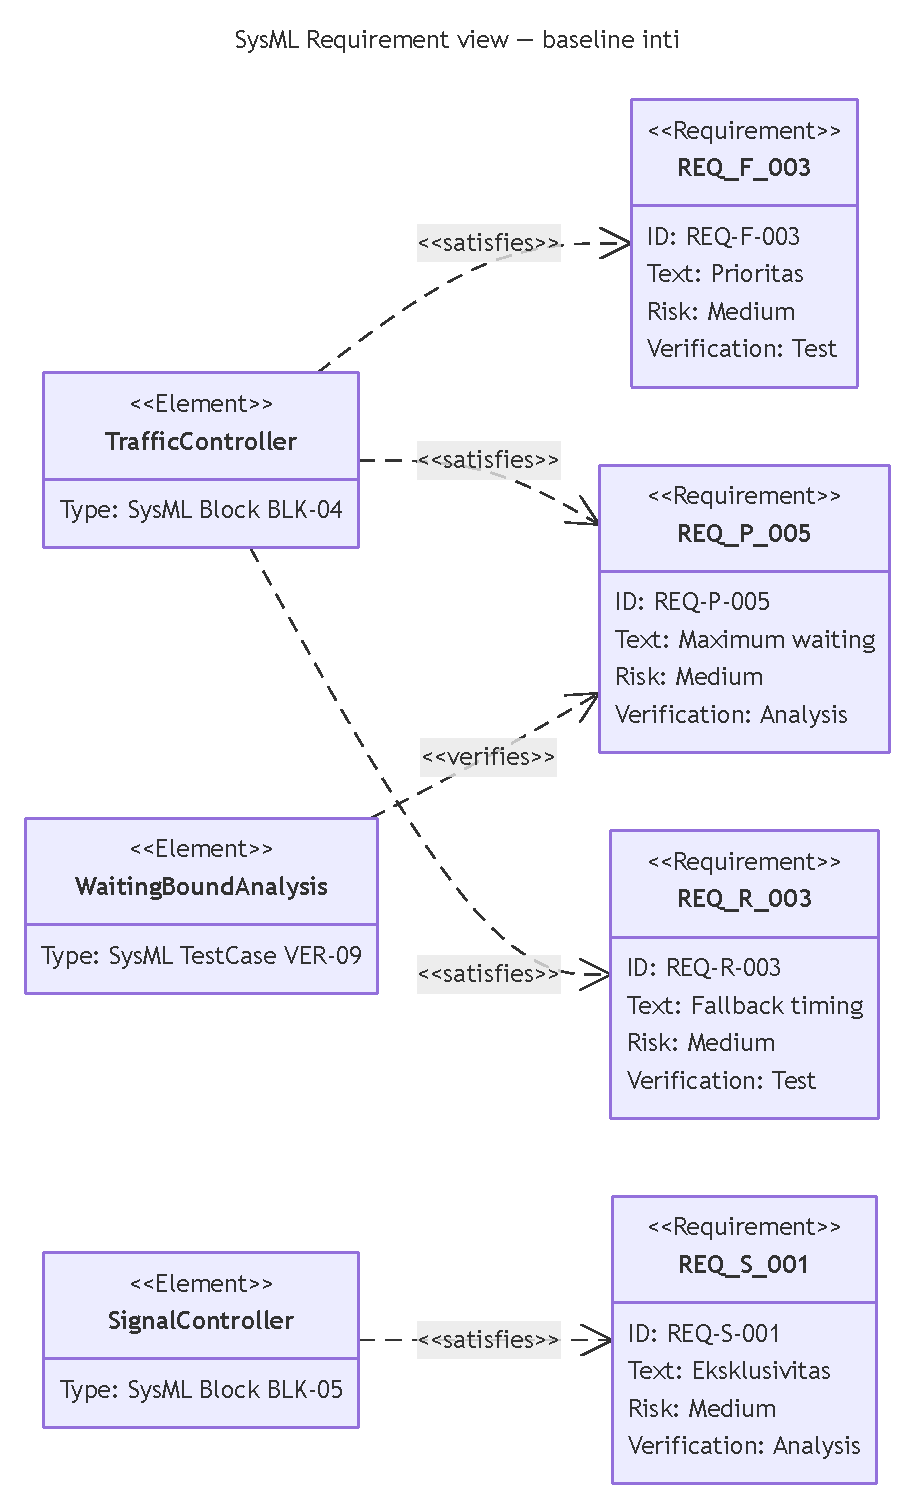
\includegraphics[width=\linewidth,height=.60\textheight,keepaspectratio]{requirements.pdf}
\caption{Requirement view dari model baseline}\label{fig:requirements}
\sumber{Pemodelan proyek berdasarkan asumsi desain ASM-001--010 (2026)}
\end{figure}
\clearpage
\clearpage
\begin{landscape}
\section{Use case view}
UC-02 mencakup MaintainSafeSignals, sedangkan HandleDataFailure memperluas pelayanan pada kondisi dataFault. TrafficDataSource tetap di luar boundary; komponen internal tidak dijadikan actor.
\begin{figure}[htbp]\centering
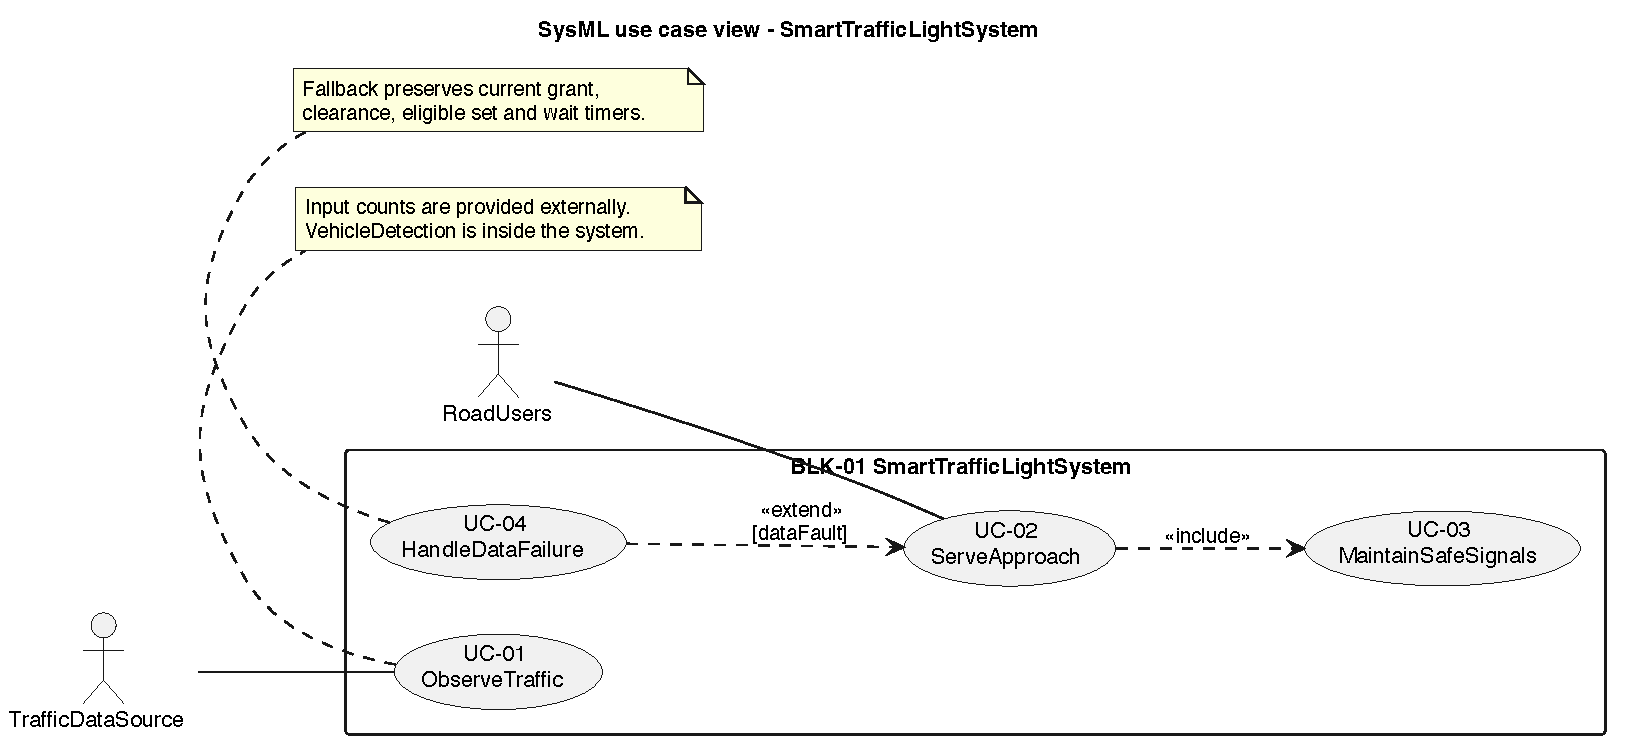
\includegraphics[width=\linewidth,height=.66\textwidth,keepaspectratio]{use-case.pdf}
\caption{Use case view dari model baseline}\label{fig:use-case}
\sumber{Pemodelan proyek berdasarkan asumsi desain ASM-001--010 (2026)}
\end{figure}
\clearpage
\end{landscape}
\clearpage
\section{Activity view}
Alokasi action ke block tercantum pada dictionary model. Loop menerima event sample atau phase timer; transisi clearance hanya berjalan bila event STM-01 mengaktifkannya, bukan delay blocking setiap sampel.
\begin{figure}[htbp]\centering
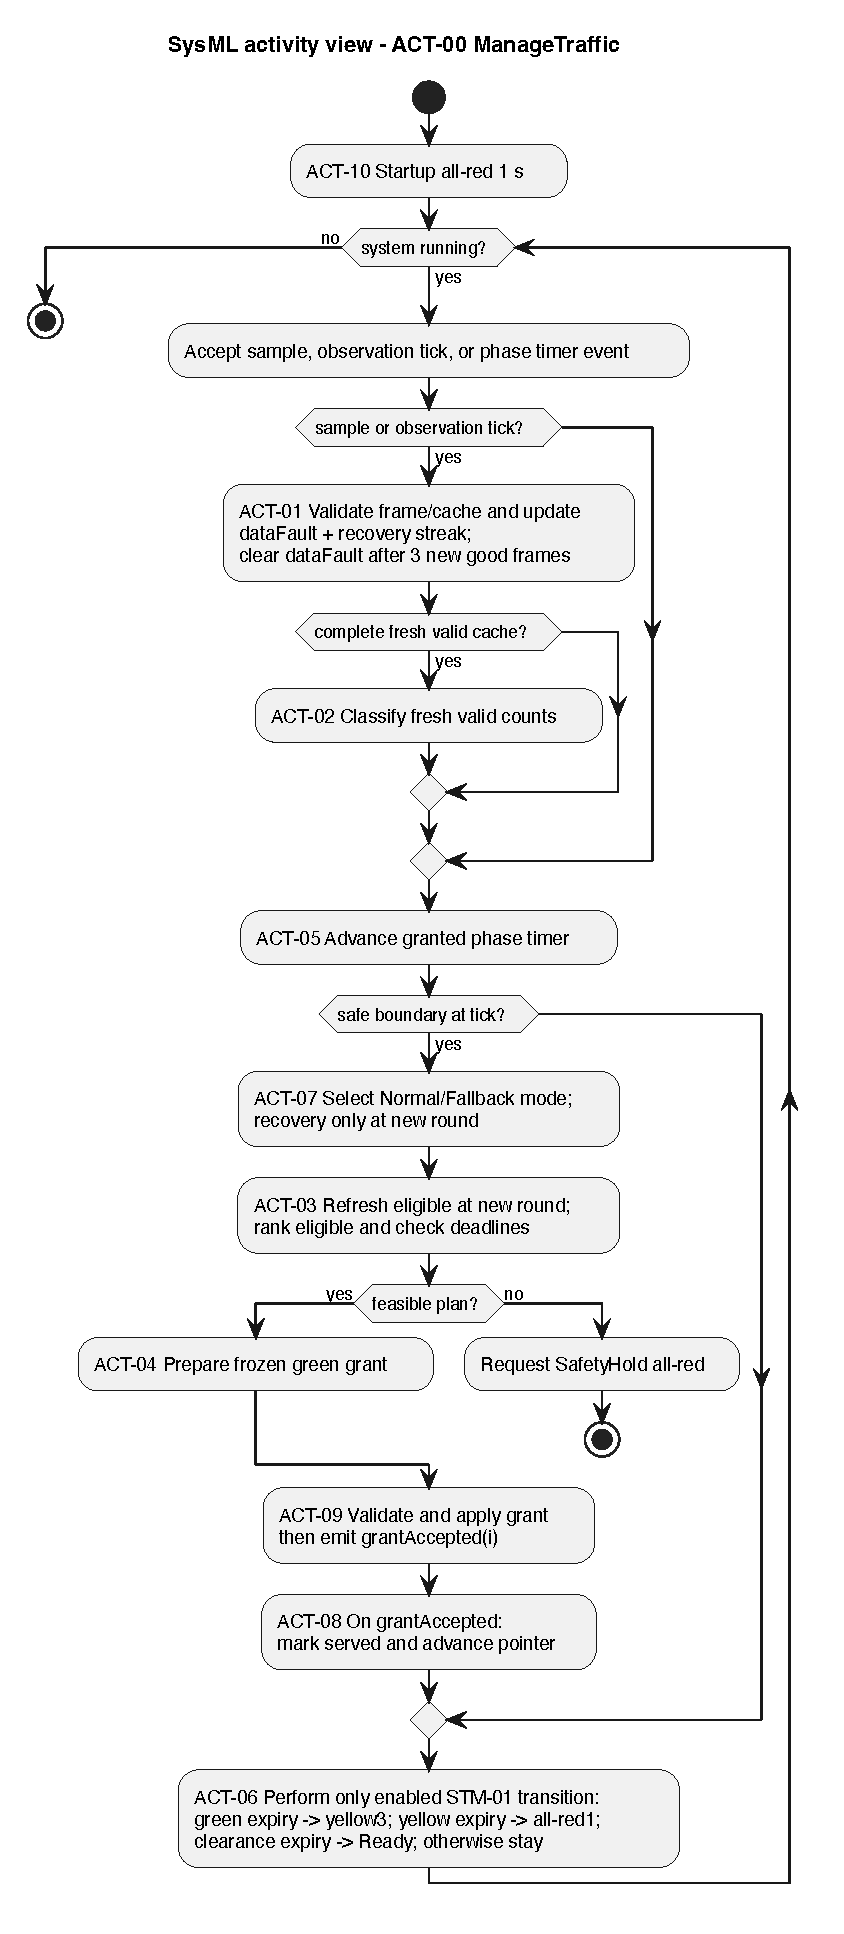
\includegraphics[width=\linewidth,height=.76\textheight,keepaspectratio]{activity.pdf}
\caption{Activity view dari model baseline}\label{fig:activity}
\sumber{Pemodelan proyek berdasarkan asumsi desain ASM-001--010 (2026)}
\end{figure}
\clearpage
\clearpage
\begin{landscape}
\section{Sequence view}
Lifeline mereferensikan part yang sama dengan IBD. DataFault dilatch selama green, tetapi grant tetap sampai timer berakhir; mode berikutnya diputuskan pada boundary aman.
\begin{figure}[htbp]\centering
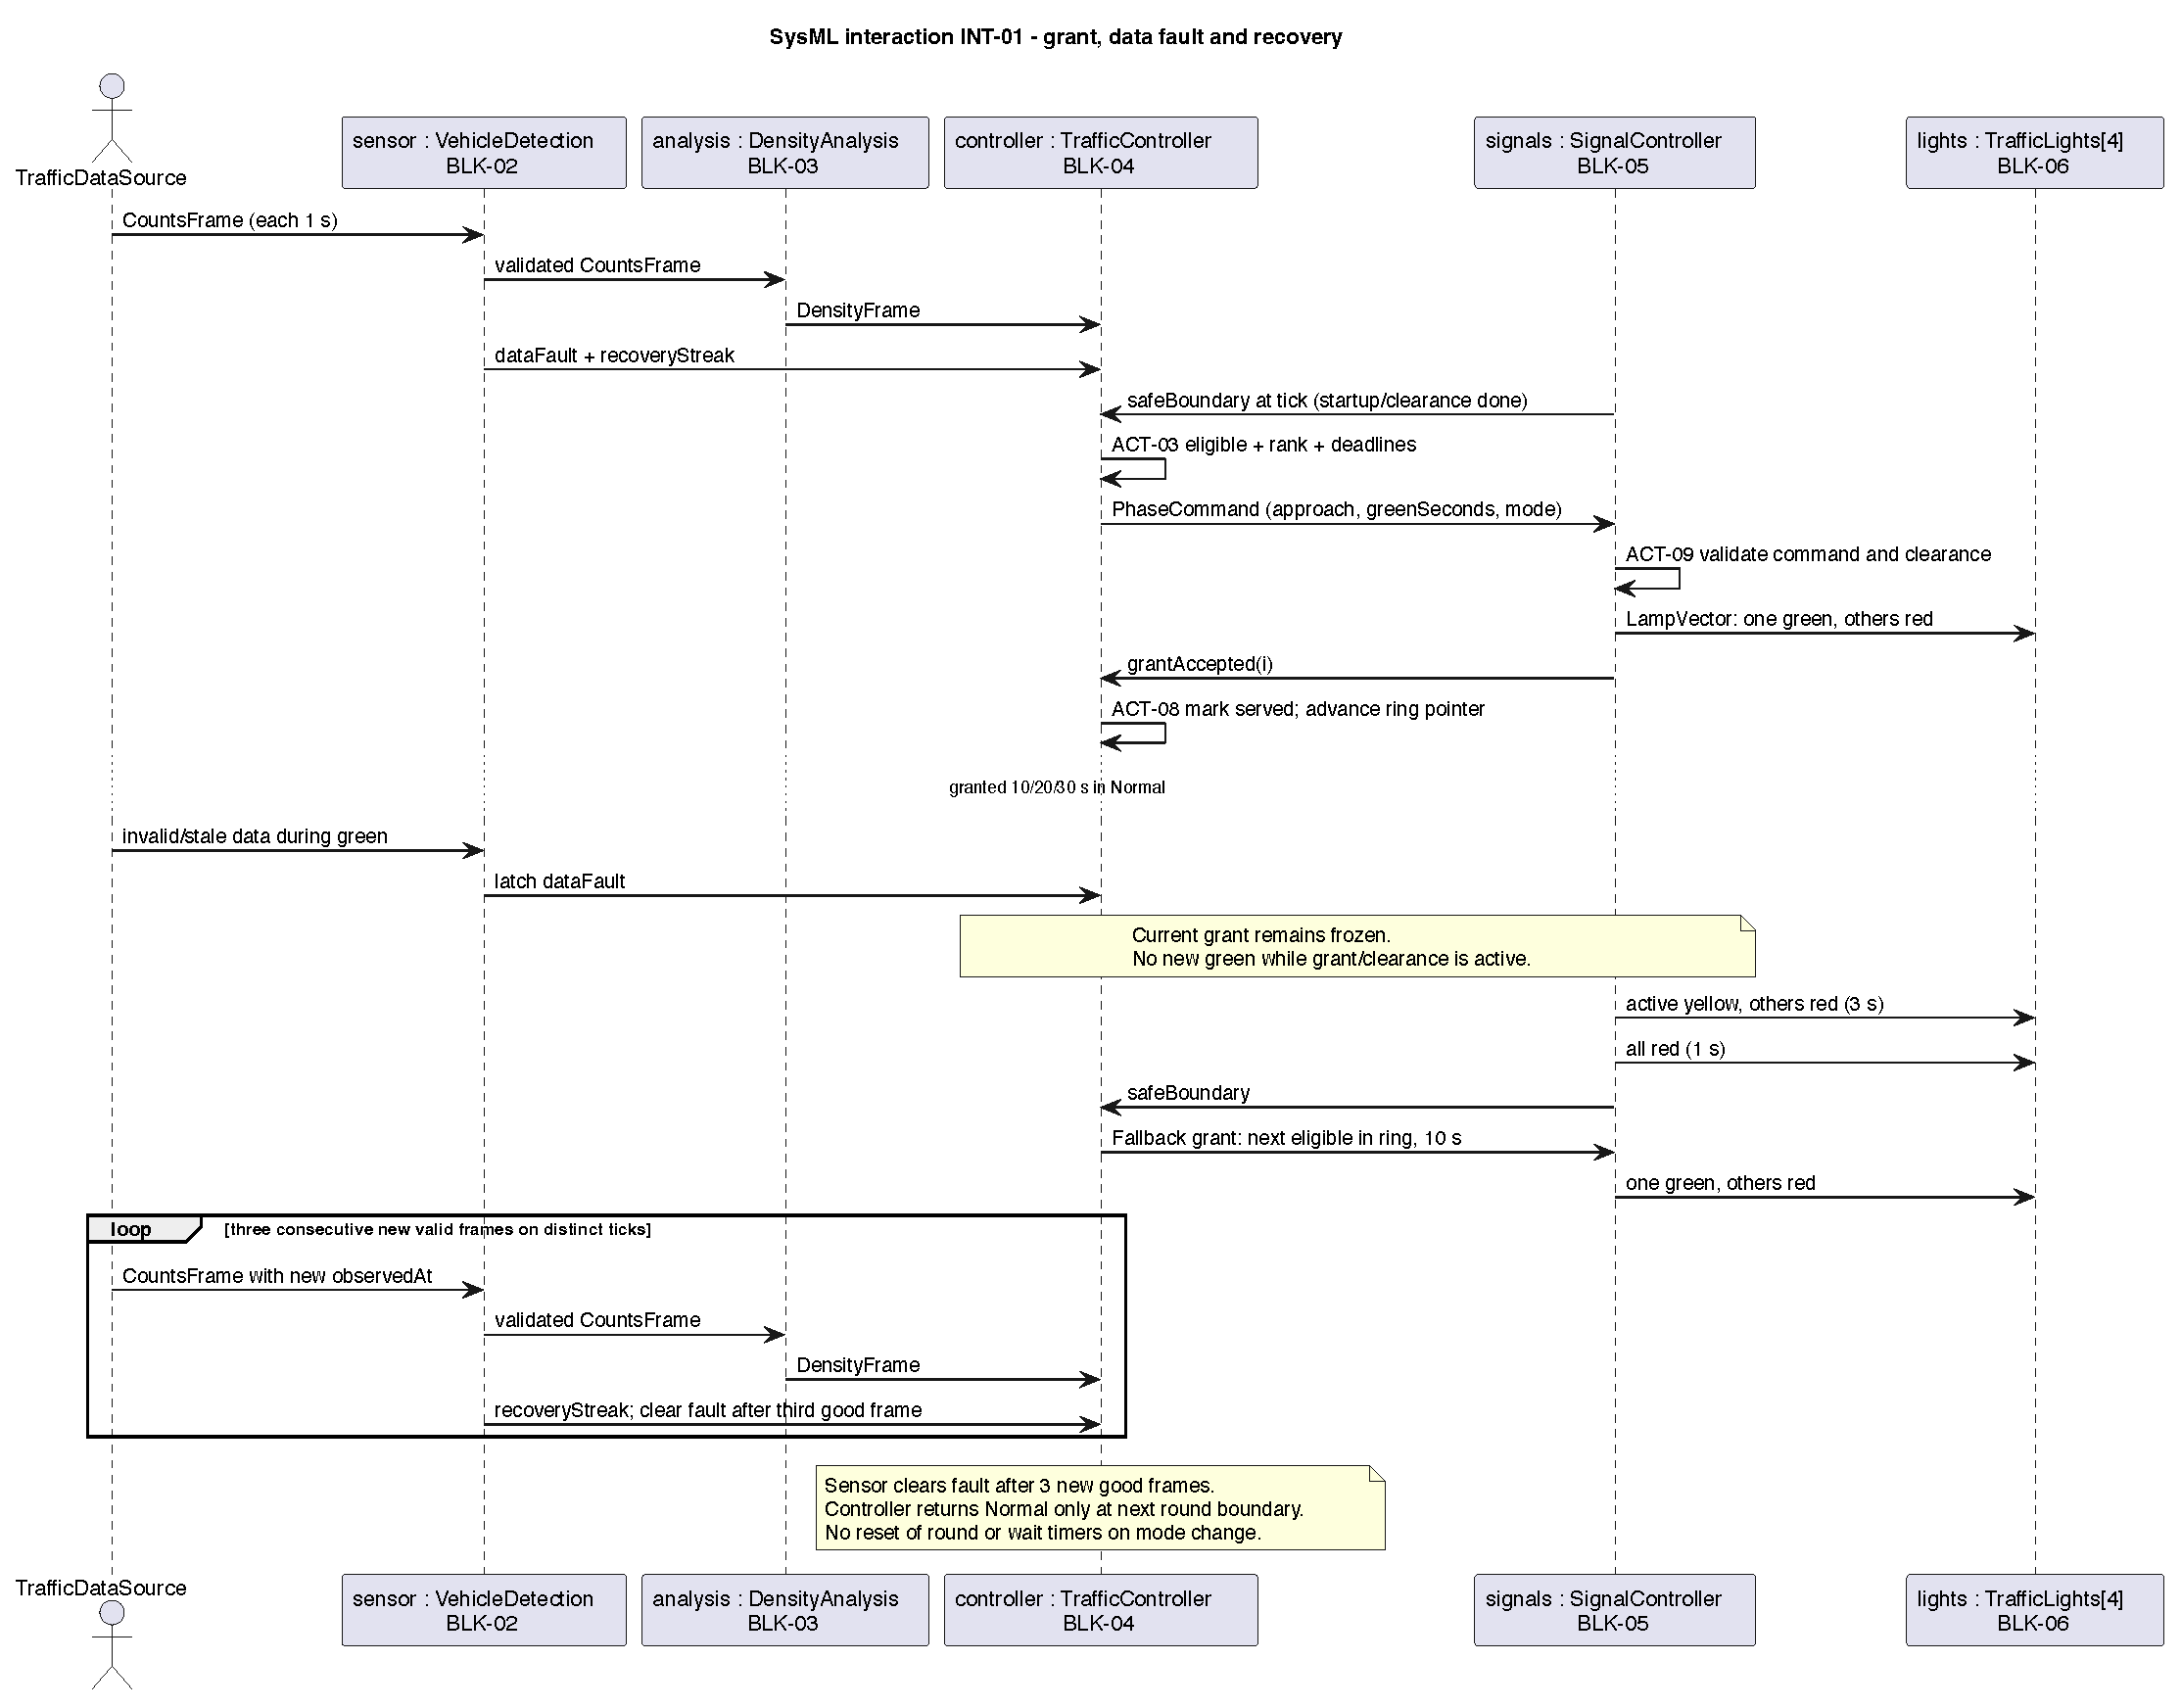
\includegraphics[width=\linewidth,height=.66\textwidth,keepaspectratio]{sequence.pdf}
\caption{Sequence view dari model baseline}\label{fig:sequence}
\sumber{Pemodelan proyek berdasarkan asumsi desain ASM-001--010 (2026)}
\end{figure}
\clearpage
\end{landscape}
\clearpage
\section{State machine view}
STM-01 dimiliki SignalController. Normal/Fallback merupakan variabel controller, bukan region sinyal concurrent. SafetyHold berada di luar composite Running dan keluar hanya melalui restart.
\begin{figure}[htbp]\centering
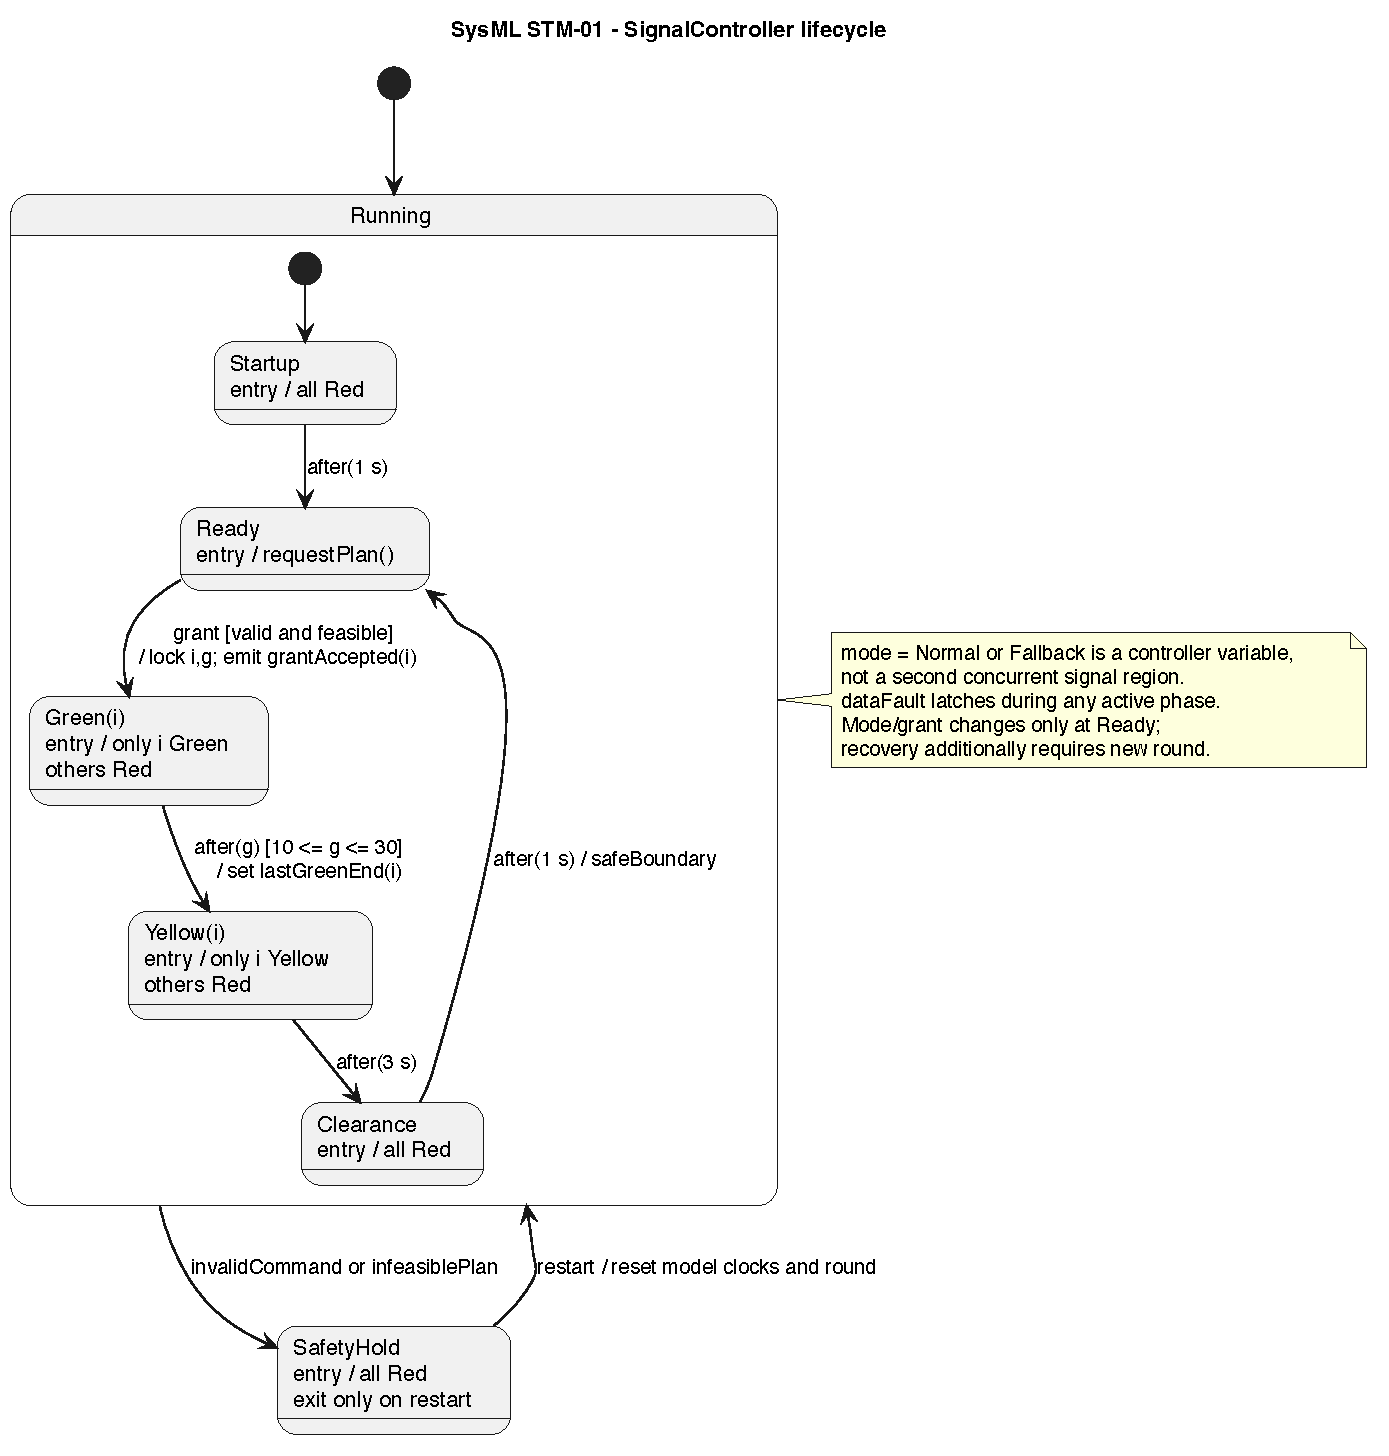
\includegraphics[width=\linewidth,height=.76\textheight,keepaspectratio]{state-machine.pdf}
\caption{State machine view dari model baseline}\label{fig:state-machine}
\sumber{Pemodelan proyek berdasarkan asumsi desain ASM-001--010 (2026)}
\end{figure}
\clearpage
\clearpage
\begin{landscape}
\section{Block Definition Diagram}
BDD mendefinisikan tipe BLK-01 sampai BLK-06 dan composition part dengan multiplicity. InterfaceBlock/value types didefinisikan dalam dictionary model; port receiver memakai conjugation.
\begin{figure}[htbp]\centering
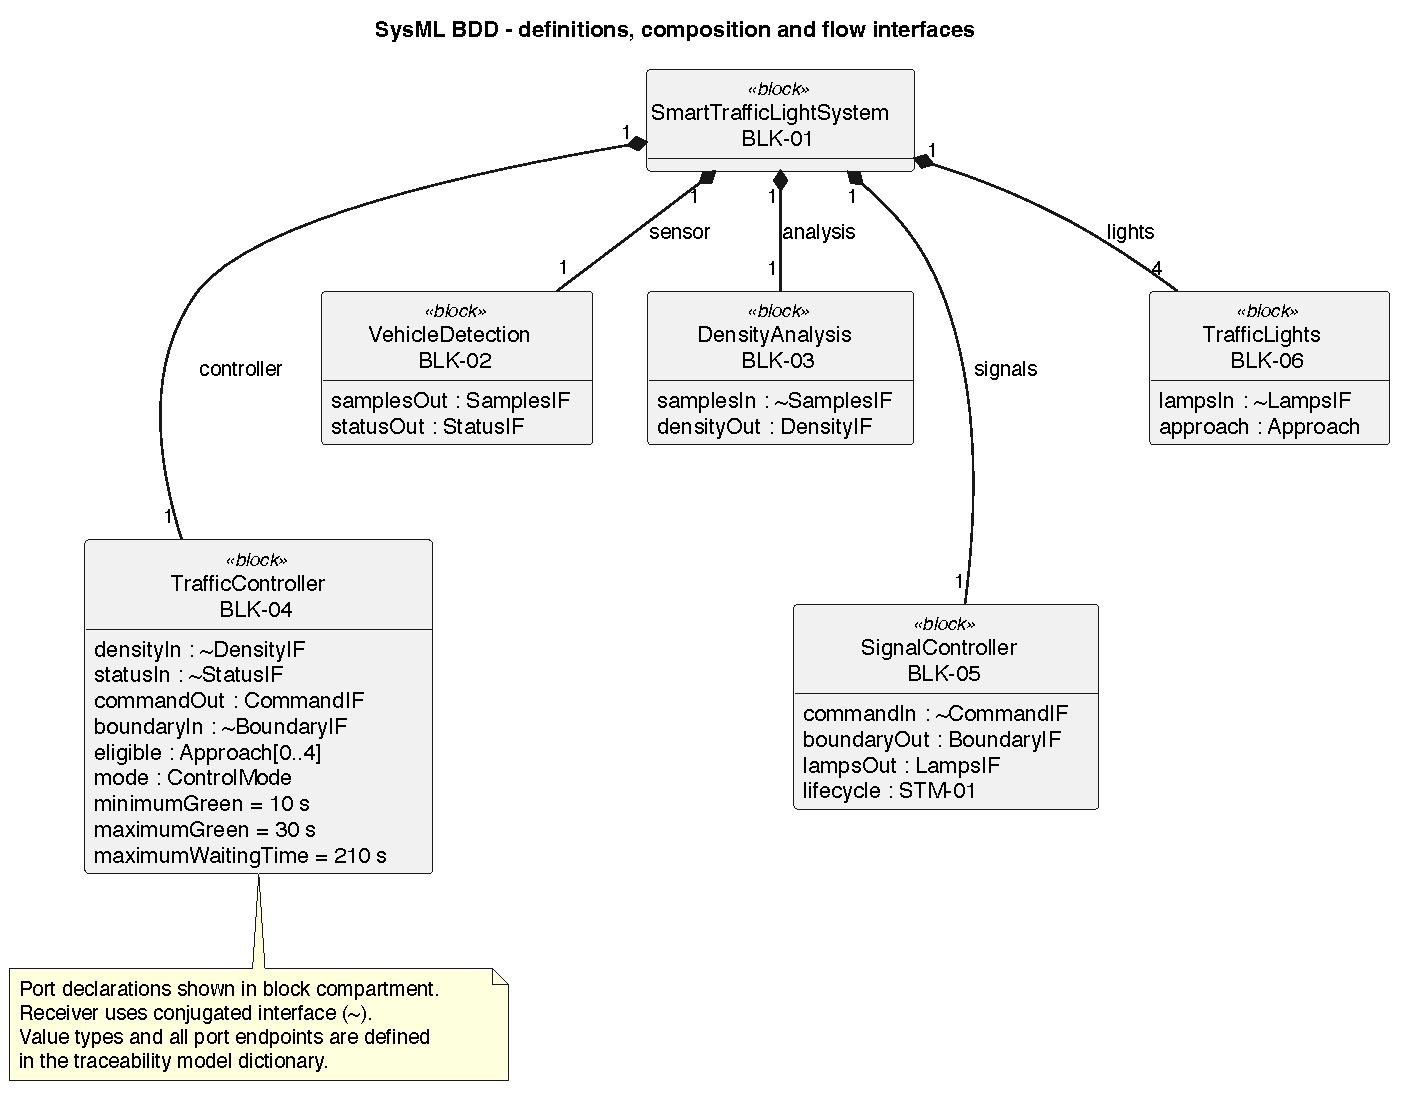
\includegraphics[width=\linewidth,height=.66\textwidth,keepaspectratio]{bdd.pdf}
\caption{Block Definition Diagram dari model baseline}\label{fig:bdd}
\sumber{Pemodelan proyek berdasarkan asumsi desain ASM-001--010 (2026)}
\end{figure}
\clearpage
\end{landscape}
\clearpage
\begin{landscape}
\section{Internal Block Diagram}
IBD memakai part dari BDD dalam context BLK-01. P01--P12 mengacu ke port bertipe pada dictionary. C01--C06 adalah assembly connector dengan item flow; panah menunjukkan flow, bukan dependency satisfy.
\begin{figure}[htbp]\centering
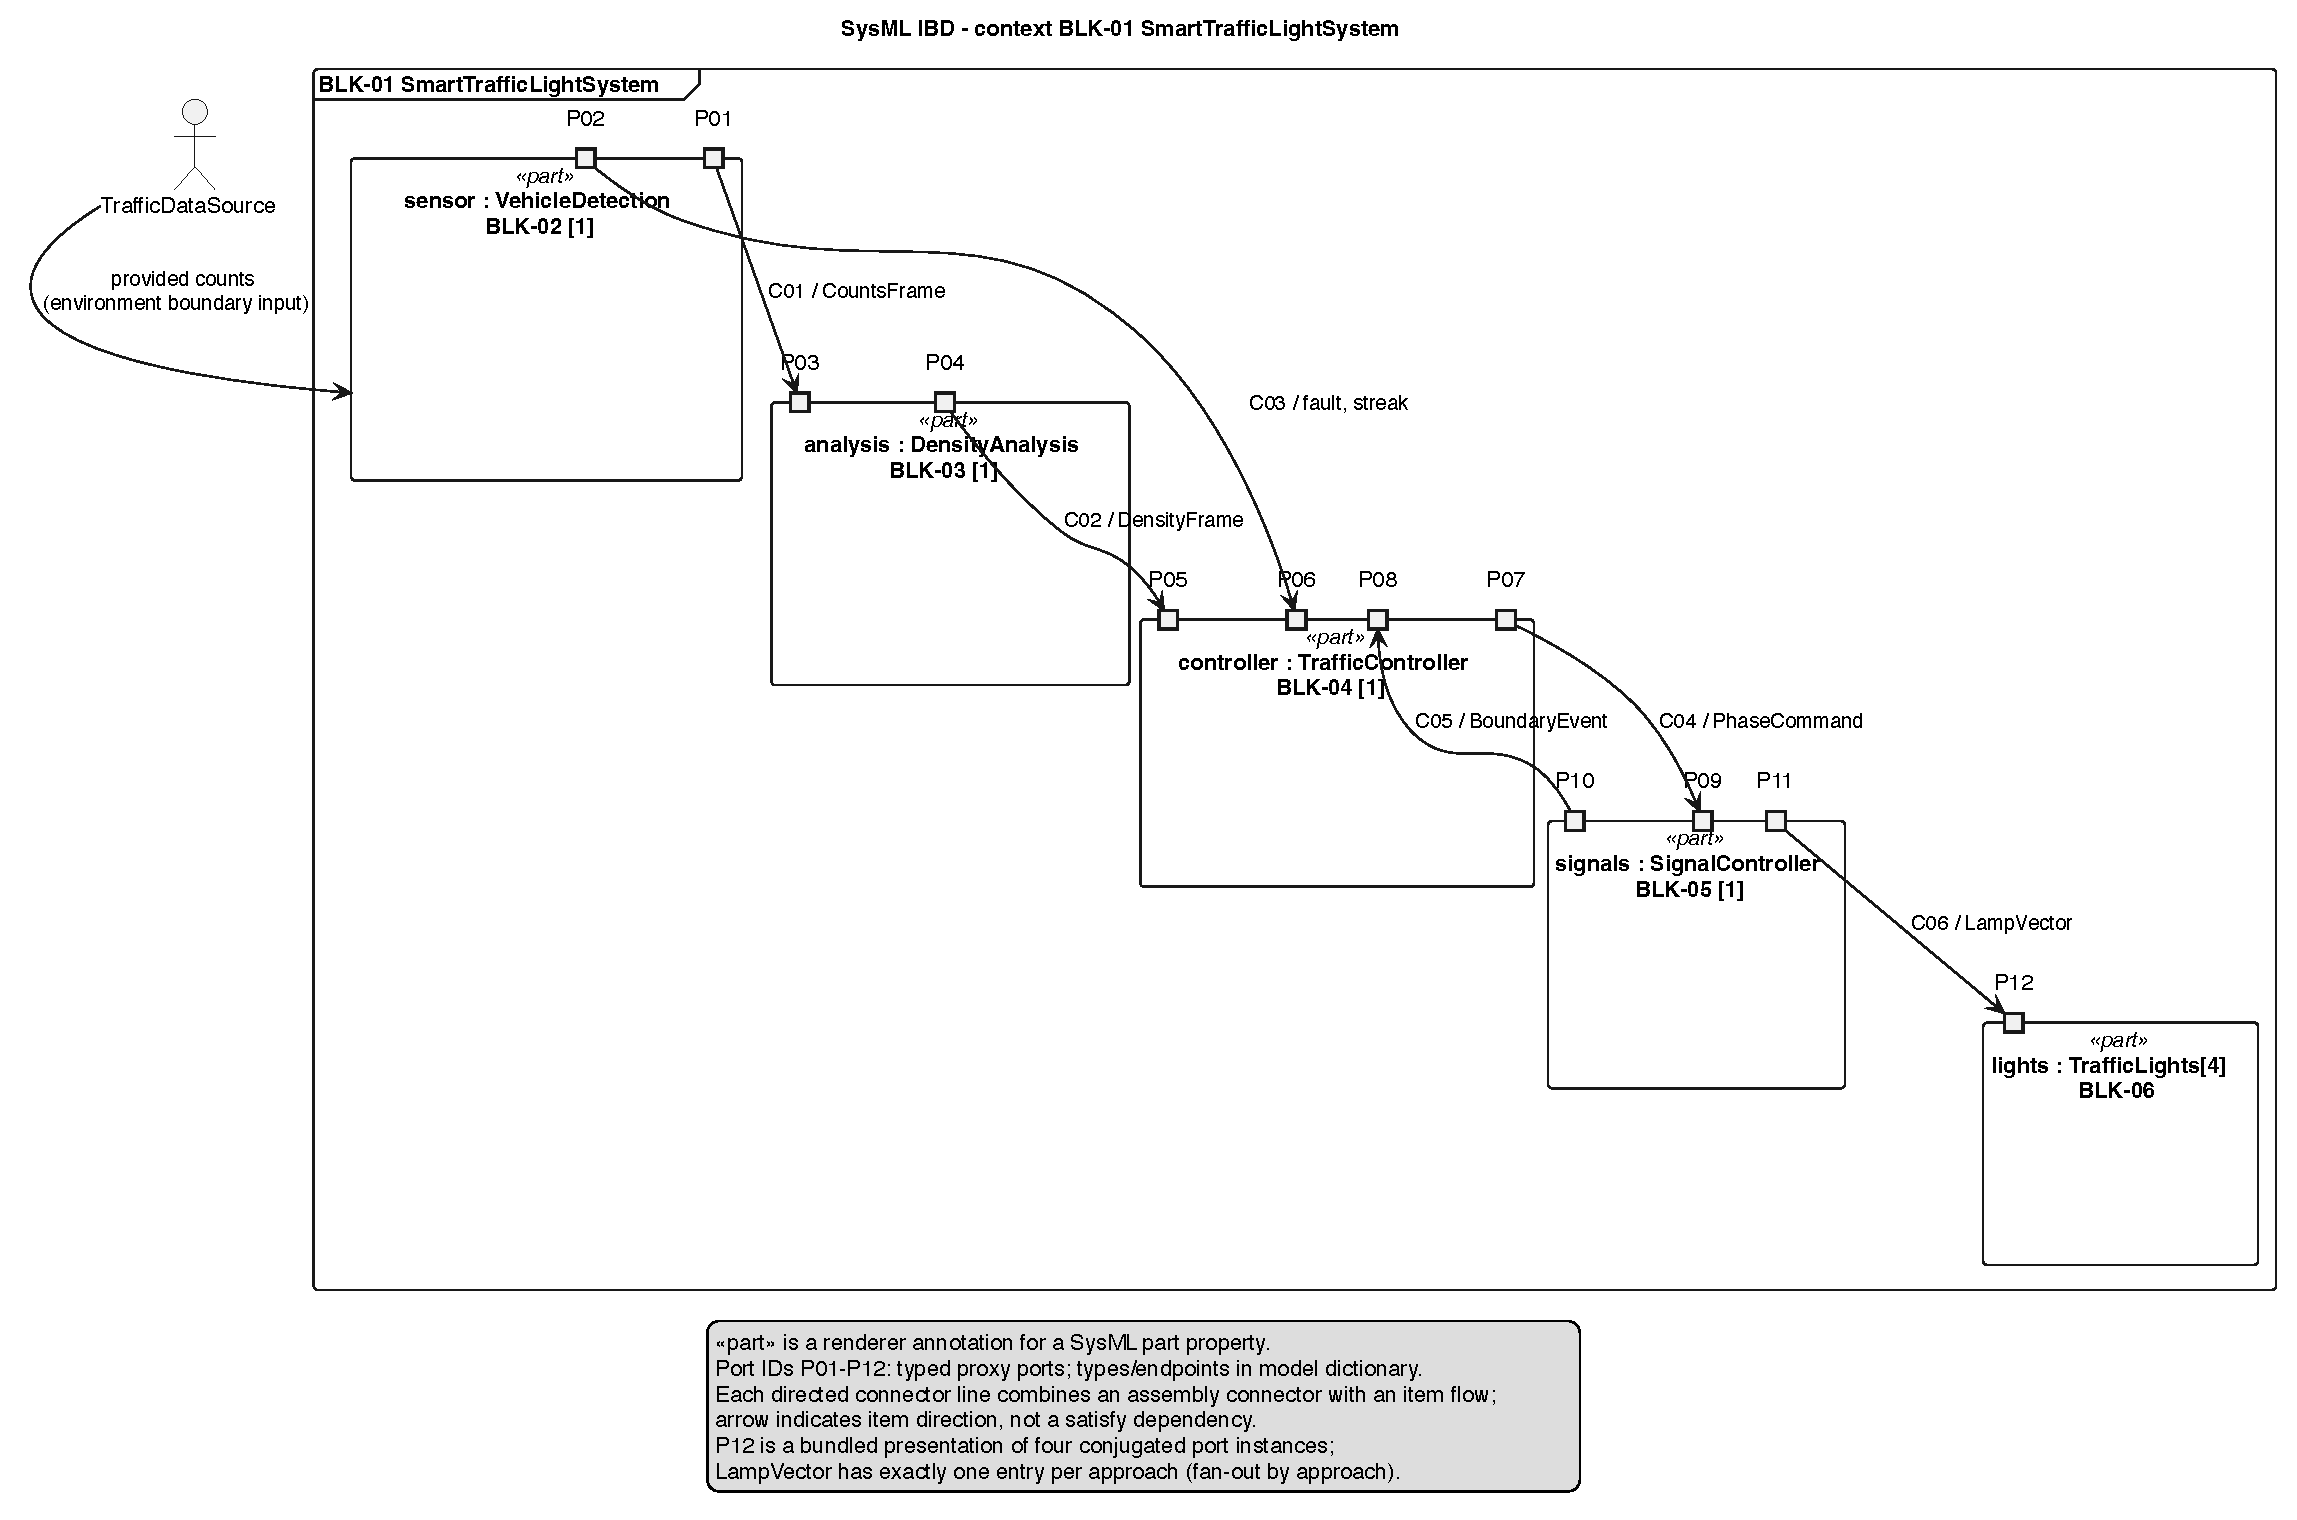
\includegraphics[width=\linewidth,height=.66\textwidth,keepaspectratio]{ibd.pdf}
\caption{Internal Block Diagram dari model baseline}\label{fig:ibd}
\sumber{Pemodelan proyek berdasarkan asumsi desain ASM-001--010 (2026)}
\end{figure}
\clearpage
\end{landscape}

\section{Traceability dan Verification Scenarios}
\subsection{Penelusuran requirement}
Matrix berikut memuat seluruh requirement. Sources tersedia pada katalog. Setiap block mengarah melalui dependency satisfy ke requirement; setiap test case melalui verify ke requirement. Action dialokasikan ke block, dengan arah allocation dari action ke block. Hubungan ini menyatakan tanggung jawab desain, bukan verdict pelaksanaan.
\begin{longtable}{lllll}
\toprule Requirement & Use case & Action & Block & TestCase \\\midrule\endhead
REQ-F-001 & UC-01 & ACT-02 & BLK-03 & VER-01 \\
REQ-F-002 & UC-02 & ACT-08 & BLK-04 & VER-02 \\
REQ-F-003 & UC-02 & ACT-03 & BLK-04 & VER-03 \\
REQ-F-004 & UC-02 & ACT-04 & BLK-04 & VER-04 \\
REQ-F-005 & UC-02 & ACT-03 & BLK-04 & VER-05 \\
REQ-P-001 & UC-01 & ACT-01 & BLK-02 & VER-06 \\
REQ-P-002 & UC-02 & ACT-03 & BLK-04 & VER-07 \\
REQ-P-003 & UC-03 & ACT-05 & BLK-05 & VER-08 \\
REQ-P-004 & UC-03 & ACT-05 & BLK-05 & VER-08 \\
REQ-P-005 & UC-02 & ACT-03 & BLK-04 & VER-09 \\
REQ-S-001 & UC-03 & ACT-05 & BLK-05 & VER-10 \\
REQ-S-002 & UC-03 & ACT-06 & BLK-05 & VER-11 \\
REQ-S-003 & UC-03 & ACT-06 & BLK-05 & VER-11 \\
REQ-S-004 & UC-03 & ACT-09 & BLK-05 & VER-12 \\
REQ-S-005 & UC-02 & ACT-03 & BLK-04 & VER-13 \\
REQ-S-006 & UC-03 & ACT-03 & BLK-04 & VER-13 \\
REQ-I-001 & UC-01 & ACT-01 & BLK-02 & VER-14 \\
REQ-I-002 & UC-03 & ACT-05 & BLK-06 & VER-15 \\
REQ-R-001 & UC-04 & ACT-01 & BLK-02 & VER-16 \\
REQ-R-002 & UC-04 & ACT-07 & BLK-04 & VER-17 \\
REQ-R-003 & UC-04 & ACT-07 & BLK-04 & VER-18 \\
REQ-R-004 & UC-04 & ACT-07 & BLK-04 & VER-19 \\
REQ-D-001 & UC-02 & ACT-03 & BLK-01 & VER-20 \\
REQ-D-002 & UC-02 & ACT-03 & BLK-01 & VER-21 \\
\bottomrule\end{longtable}
\subsection{Interface internal}
Proxy port bertipe InterfaceBlock; port penerima dikonjugasikan. Connector C01 membawa CountsFrame dari sensor ke analysis, C02 DensityFrame dari analysis ke controller, C03 fault/streak dari sensor ke controller, C04 PhaseCommand dari controller ke signals, C05 BoundaryEvent (SafeBoundary atau GrantAccepted) dari signals ke controller, dan C06 LampVector ke empat lights. Setiap light memiliki approach yang berbeda dan mengambil entry vector yang sesuai. Annotation part dan port PlantUML tidak diklaim sebagai validasi native SysML.
\subsection{Skenario dan receipt pelaksanaan}
Sebanyak 21 test case didefinisikan dalam source verification. Cakupan meliputi kategori, sekali pelayanan per round, tie/ring, grant freeze, wait timer, cadence, boundary, min/max green, fairness, exclusivity, clearance, command rejection, deadline override, domain input, output flow, stale, fault, fallback, recovery, scope dan semantik SysML. Setiap skenario memuat kondisi awal, stimulus/timeline, expected behavior, kriteria lulus/gagal dan metode.
Checker referensi \texttt{model/verification/check\_model.py} benar-benar dijalankan. Ia tidak mengeksekusi source diagram atau perangkat fisik. Hasil yang tersedia diringkas pada Tabel~\ref{tab:results}.
\begin{table}[htbp]\centering\small
\caption{Hasil analisis yang dijalankan dan batas cakupannya.}\label{tab:results}
\begin{tabular}{lp{.70\linewidth}}\toprule TestCase & Evidence aktual \\\midrule
VER-01,03 & Contoh boundary kategori, tie/ring/wait/category pada fungsi referensi \\
VER-09 & 576 pasangan permutasi, 2304 service waits, maksimum 208 s; startup 103 s \\
VER-10 & Sembilan vector output state, masing-masing paling banyak satu Green \\
VER-13 & Contoh aritmetika deadline nominal gagal, EDF layak, deadline sudah terlewat \\
VER-14 & Predikat referensi menolak count/ID/timestamp/validity salah \\
VER-16 & Umur 3 fresh, umur 4 stale; transisi mode belum dieksekusi \\
Cross-links & 24 ID requirement unik, sumber dan 21 definisi verification terlacak \\\bottomrule
\end{tabular}\end{table}
VER-02/04/05/06/07/08/11/12/17/18/19 tetap not-run sebagai dynamic/complete inspections pada receipt executable. Expected timeline tersedia, tetapi tidak dipromosikan menjadi measured result. VER-15/20/21 diperiksa secara terpisah pada source dan dicatat dalam manual-inspection.md. Pemeriksaan semantik terpisah pada dictionary/model dilakukan secara inspection source dan tidak mengubah klaim cakupan eksekusi checker.
\subsection{Contoh timeline konseptual}
Jika N mendapat green pada t=1 sampai 11, perubahan kategori pada t=2 tidak mengubah grant tersebut. Yellow berlangsung 11--14, all-red 14--15, dan green berikutnya paling awal 15. Jika dataFault muncul saat grant 30 s pada t=5, green N berakhir 31, yellow 31--34, all-red 34--35, lalu Fallback memberi green 10 pada boundary 35. Ini expected behavior dari kontrak, bukan hasil runtime controller.
Pemulihan menuntut tiga timestamp baru yang valid dan round baru. Retransmisi timestamp yang sama tidak meningkatkan streak. Deadline precedence diuji secara aritmetika: pada t=200, melayani N selama 30 s ditambah clearance 4 akan membuat S dengan deadline 210 mulai 234; urutan EDF dapat memilih S pada 200. Jika deadline sudah terlewat sebelum keputusan, tidak ada pengurutan yang mengembalikannya dan SafetyHold diminta.

\chapter{Diskusi}
\section{Konsistensi dan keterbatasan model}
Model menghubungkan alasan desain ke requirement dan memisahkan definisi block dari pemakaian part. Ringkasan diagram tidak mengubah statement katalog, dan arah satisfy/verify mengikuti standar. Namun textual rendering tools tidak menyediakan seluruh validasi semantik SysML; inspection source dan dictionary tetap diperlukan. Tidak ada klaim sertifikasi formal atau kemampuan interchange model.

Aturan sekali pelayanan per round memberi bound analitis yang mudah diaudit, tetapi mengharuskan pelayanan count nol dan membatasi optimasi throughput. Kategori mengkuantisasi data: dua hitungan berbeda dapat memperoleh durasi sama. Prioritas density hanya berlaku pada eligible, sehingga ruas padat tidak mengulang pelayanan dalam round yang sama. Tradeoff ini dipilih untuk fairness konseptual, bukan dinyatakan optimal oleh jurnal.

Bound 208 s bergantung pada clock ideal, green maksimal 30, clearance 4 dan empat pelayanan per round. Bound tersebut bukan jaminan individual queue delay, antrean habis, atau kapasitas lokasi. SafetyHold/restart mengecualikan bound, dan actuator/listrik/network failure di luar fault model. Perlu kalibrasi geometri, detector, clearance, latensi dan validasi lapangan sebelum aplikasi fisik. Proyek ini tidak membuat deployment tersebut.

\section{Integritas evidence dan langkah lanjutan}
Klaim 31.05\%,96\%,90\% berasal dari artikel dan tidak menjadi hasil proyek. Artikel traffic memiliki perbedaan konteks serta istilah yang didisposisikan; kajian MBSE tidak membuktikan penghematan kausal proyek. Akses penerbit dan peringatan xref lokal tetap dinyatakan. Catatan kuliah yang diperluas tidak diatribusikan sebagai slide asli yang sudah dicocokkan. Seluruh file jurnal pengguna dipertahankan.

Langkah lanjutan yang bermakna adalah mengimplementasikan scheduler/phase engine dan menjalankan timeline fault/recovery, kemudian menguji detector dan perangkat lampu pada lingkungan yang sesuai. Analisis throughput memerlukan simulator, skenario input, pembanding dan data yang dapat direplikasi; itu belum dilakukan. Tidak perlu menambah ML atau emergency preemption hanya untuk memperbanyak fitur.

\chapter{Kesimpulan}
Proyek menghasilkan model konseptual Smart Traffic Light dengan 24 requirement dan tujuh view SysML, serta traceability ke 21 skenario. Receiver count, klasifikasi kategori, scheduler round, signal lifecycle dan output lampu memiliki tanggung jawab serta interface yang jelas. Parameter baseline merupakan asumsi desain yang dapat diubah dengan revisi terkontrol. Pemeriksaan referensi menghasilkan bound service waiting 208 s pada 576 pasangan urutan round, di bawah batas 210 s, dan memeriksa contoh input/tie/output-state. Hasil ini terbatas pada kontrak model; fault/recovery penuh, traffic throughput dan keselamatan hardware belum diverifikasi. Laporan tidak menyamakan keberhasilan build dengan bukti eksperimen fisik.

\daftarreferensi
\end{document}
